
In this chapter, we specify a generative model for transcript quantification from long-read direct \gls{rnaseq} that accounts for bias due to degradation of \gls{mrna} transcripts. We detail the assumptions of our model, formulate the generative process and derive statistical algorithms for inference of the parameters of the model.  

\section{Model assumptions}\label{sec:model-assumptions}

The input to our model consists of reads obtained from sequencing transcripts with the \gls{ont} direct \gls{rnaseq} protocol aligned to the reference transcriptome. We assume there is a bijective mapping between reads and transcript, i.e., each read originates from only one transcript, and each transcript generates only one read. Reads are generated independently and identically distributed (iid) from a distribution to be specified, and the 3' end of each read aligns within some region close to the 3' end of the isoform it originated from.

We make two assumptions on the degradation rate $d$. First, we assume that the degradation of a transcript does not depend on the expression level or biotype of the isoform it originated from. Second, we assume that the expected degradation rate is constant, i.e, $\mathbb{E}[d]=c\in(0,1)$. Even though the second assumption is relatively strong (see Section \ref{sec:read-length-isoform-agreement}), we make this simplifying assumption to show that our model works on simulated data, and relax this assumption to allow our model to generalize to real datasets. 

\section{Generative model}\label{sec:generative-model}

Our model aims to capture the generative process of the observed degraded reads from their isoforms of origin. Here, we formalize our model and derive the complete data log likelihood for maximum likelihood estimation of the model parameters. 

\subsection{Notation and formulation}\label{sec:notation-and-formulation}

Let $N$ be the number of observed reads and $M$ be the number of isoforms the reads were generated from. 
\begin{itemize}
    \item We observe a set of reads $\bm{R}=\{r_1,...,r_N\}$, with $r_i$ representing the $i$\ts{th} read. The variable $r_i$ can be thought of as a collection of properties about the $i$\ts{th} read that are relevant for quantification, such as length, start and end positions or GC content.
    \item Our goal is to infer the unknown relative abundances of the isoforms $\bm{\theta}=\{\theta_1,...\theta_M\}$. These relative abundances sum to one and are non-negative, i.e., $\Sigma_j\theta_j=1, \theta_j\geq0$ $\forall j$. 
    \item We introduce $N$ latent variables $\bm{Z}=\{z_1,...,z_N\}$, where $z_i=(z_{i1}$ $...$ $z_{iM})^T$ is a binary vector in $M$-dimensions with $\Sigma_jz_{ij}=1$. $z_i$ describes the assignment of $r_i$ to one of $M$ isoforms, where
    \begin{equation}
        z_{ij} = 
        \begin{cases}
        1 & \text{if } r_i \text{ originated from isoform } j\\
        0 & \text{otherwise }
        \end{cases}
    \end{equation}
\end{itemize} 
The directed graphical model in Figure \ref{fig:graphical-model-1} illustrates the relationship between the variables $\bm{R}, \bm{Z}$ and parameters $\bm{\theta}$, and provides an easy way to read off the factorization of the joint distribution over the observed and latent variables:
\begin{equation}
    p(\bm{R},\bm{Z})=p(\bm{R}\mid\bm{Z})\cdot p(\bm{Z})\label{eq:joint-dist}
\end{equation}
\begin{figure}[H]
    \centering
    \begin{tikzpicture}[scale=1.25, every node/.style={transform shape}]
        \node[const](theta){$\bm{\theta}$}; % 
        \node[latent, right=of theta](z){$z_i$}; %
        \node[obs, right=of z](r){$r_i$}; %
        \edge{theta}{z}; %
        \edge{z}{r}; %
        \plate[inner sep=0.4cm, xshift = -0.1cm]{plate1}{(z)(r)}{$i=1,...,N$}; %
    \end{tikzpicture}
    \caption[Graphical model for long-read RNA-seq]{Graphical model for long-read RNA-seq. Nodes are random variables, and directed edges represent the dependencies between them. Shaded nodes are observed, while unobserved nodes are latent. Variables within the plate are replicated $N$ times.}
    \label{fig:graphical-model-1}
\end{figure}
\noindent The distribution over the latent variables is categorical:
\begin{equation}
    p(z_i)=\prod_{j=1}^M \theta_j^{z_{ij}}\label{eq:latent-dist}
\end{equation}
The conditional distribution of observing the read $r_i$ given $z_i$ is
\begin{equation}
    p(r_i\mid z_i)=\prod_{j=1}^M p(r_i\mid z_{ij})^{z_{ij}}\label{eq:cond-dist}
\end{equation}
We now model the probability that read $i$ originated from isoform $j$, i.e., $p(r_i\mid z_{ij}=1)$. This probability is proportional to:
\begin{itemize}
    \item The alignment compatibility $a_{ij}\in(0,1)$ between read $i$ and isoform $j$, which measures the alignment score (AS) of read $i$ against isoform $j$ scaled by the best alignment score of read $i$ against all isoforms:
    \begin{equation}
        a_{ij} = \frac{{\textrm{AS}}_{ij}}{\max_{j'} {\textrm{AS}}_{ij'}}
    \end{equation}
    \item The probability of observing a read of length $\ell_i$ given the degradation rate $d_j$ of isoform $j$, i.e., $p(\ell_i\mid d_j, \mathrm{len}(j), z_{ij}=1)$, where $\ell_i$ is the length of $r_i$. We refer to this probability as the \textit{read length-isoform agreement} model.      
\end{itemize}
Combining alignment compatibility and the read length-isoform agreement model, we have 
\begin{equation}
    p(r_i\mid z_{ij}=1) = a_{ij}\cdot p(\ell_i\mid d_j, z_{ij}=1)\label{eq:read-iso-agreement}
\end{equation}
We make some remarks on equation \ref{eq:read-iso-agreement}. First, $a_{ij}$ measures how well read $i$ aligns to isoform $j$ compared to its best alignment. Note that if we do not observe an alignment between read $i$ and isoform $j$, then $\mathrm{AS}_{ij}=0$, $a_{ij}=0$, and thus $p(r_i\mid z_{ij}=1)=0$ as expected. Second, the read length-isoform agreement model captures the expected read length distribution for isoform $j$ given its degradation rate and length. In the absence of degradation, we expect that the lengths of all reads originating from isoform $j$ will be equal to the length len$(j)$ of isoform $j$, i.e., $p(\ell_i=\mathrm{len}(j)\mid d_j, z_{ij}=1)=1$ and $0$ otherwise.   

\subsection{Read length-isoform agreement}\label{sec:read-length-isoform-agreement}

We specify the read length-isoform agreement model with the assumption that the expected degradation is constant, i.e., $\mathbb{E}[d]=c\in(0,1)$. For example, if the degradation rate for all transcripts is $d_j=0.2$, then for every kb from the 3' end, we expect 20\% less reads. A constant expected degradation rate  implies that the maximum possible sequenced read length $\ell_\mathrm{max}$ is bounded, and is given by:
\begin{equation}
    -c\cdot \ell_\mathrm{max} + 1 = 0 \implies \ell_\mathrm{max} = 1/c
\end{equation}
For instance, a $\mathbb{E}[d]=0.2$ implies that $\ell_\mathrm{max}=5$ kb. The assumption made here is unrealistic, given that \gls{ont} devices are capable of sequencing reads upwards of $10$ kb in length. Nevertheless, this simplifying assumption enables us to test a simpler read length-isoform agreement model on simulated datasets. We develop a more flexible model allowing for variable degradation in the following section.  

Let the length of isoform $j$ be len$(j)$. For constant expected degradation, we have
\begin{equation}
    p(\ell_i\mid d_j, z_{ij}=1) = 
    \begin{cases}
        d_j\cdot\ell_i & \textrm{if } \ell_i<\min(\mathrm{len}(j), \ell_\mathrm{max})\\
        1-d_j\cdot\ell_i & \textrm{if } \ell_i=\mathrm{len}(j)
    \end{cases}
\end{equation}

\subsection{Likelihood formulation}\label{sec:likelihood-formulation}

The marginal distribution of $r_i$ is obtained by summing the joint distribution (Eq. \ref{eq:joint-dist}) over all $M$ possible states of $z_i$. From Eqs. \ref{eq:latent-dist}, \ref{eq:cond-dist} and \ref{eq:read-iso-agreement}, we obtain
\begin{equation}
    p(r_i)=\sum_{z_i}p(z_i)\cdot p(r_i\mid z_i)=\sum_{j=1}^M \theta_j\cdot a_{ij}\cdot p(\ell_i\mid d_j, z_{ij}=1)
\end{equation}
Since we assume the reads are generated iid, the likelihood is a product over $N$ reads:
\begin{equation}
    p(\bm{R}\mid\bm{\theta}) = \prod_{i=1}^N \sum_{j=1}^M \theta_j\cdot a_{ij}\cdot p(\ell_i\mid d_j, z_{ij}=1)\label{eq:lik}
\end{equation}
The corresponding log-likelihood is 
\begin{equation}
    \log p(\bm{R}\mid\bm{\theta}) = \sum_{i=1}^N \log \left[\sum_{j=1}^M \theta_j\cdot a_{ij}\cdot p(\ell_i\mid d_j, z_{ij}=1)\right]\label{eq:log-lik}
\end{equation}
It is difficult to maximize Eq. \ref{eq:lik} with respect to $\bm{\theta}$ because the log acts on the sum. If we had access to the latent variables $\bm{Z}$, the likelihood will decompose. To demonstrate this, we write the complete data likelihood as
\begin{equation}
    p(\bm{R},\bm{Z}\mid\bm{\theta})=\prod_{i=1}^N\prod_{j=1}^M \theta_j^{z_{ij}}\cdot\left[a_{ij}\cdot p(\ell_i\mid d_j, z_{ij}=1)\right]^{z_{ij}}\label{eq:comp-lik}
\end{equation}
The corresponding complete data log-likelihood is 
\begin{equation}
    \log p(\bm{R},\bm{Z}\mid\bm{\theta})=\sum_{i=1}^N\sum_{j=1}^M z_{ij}\cdot\log \left[\theta_j\cdot a_{ij}\cdot p(\ell_i\mid d_j, z_{ij}=1)\right]\label{eq:comp-log-lik}
\end{equation}

\section{Parameter inference}

We describe two strategies to infer the parameters $\bm{\theta}$ that maximize the likelihood of the observed data: expectation maximization and variational Bayesian inference.  

\subsection{Expectation maximization}\label{sec:em}

The EM algorithm is a powerful method for finding maximum likelihood estimates of parameters in latent variable models. It consists of a two-stage iterative optimization procedure for maximizing the likelihood. In our setting, we seek to maximize the complete data log-likelihood with respect to $\bm{\theta}$. However, we observe only the incomplete data $\bm{R}$. Since we cannot obtain the complete data log-likelihood (Eq. \ref{eq:comp-log-lik}), we take its expectation under the posterior of the latent variables $\bm{Z}$ given some setting of the parameters $\bm{\theta}^{(t)}$: this corresponds to the E step of the EM algorithm. In the M step, we maximize this expectation with respect to the parameters $\bm{\theta}$ to obtain a new estimate of the parameters $\bm{\theta}^{(t+1)}$.   

We obtain the posterior of the latent variables $\bm{Z}$ from Eqs. \ref{eq:latent-dist} and \ref{eq:joint-dist}:
\begin{equation}
    p(\bm{Z}\mid\bm{R},\bm{\theta})\propto\prod_{i=1}^N\prod_{j=1}^M\left[\theta_j\cdot a_{ij}\cdot p(\ell_i\mid d_j,z_{ij})\right]^{z_{ij}=1}\label{eq:post}
\end{equation}
\paragraph{E-step} We take the expectation of the complete data log-likelihood (Eq. \ref{eq:comp-log-lik}) with respect to the posterior distribution of the latent variables (Eq. \ref{eq:post}):
\begin{equation}
    \mathbb{E}_{\bm{Z}\mid\bm{R},\bm{\theta}}\left[\log p(\bm{R},\bm{Z}\mid\bm{\theta})\right]=\sum_{i=1}^N\sum_{j=1}^M \mathbb{E}[z_{ij}]\cdot\log \left[\theta_j\cdot a_{ij}\cdot p(\ell_i\mid d_j, z_{ij}=1)\right]\label{eq:e-step}
\end{equation}
where 
\begin{equation}
    \mathbb{E}[z_{ij}]=\frac{\theta_j\cdot a_{ij}\cdot p(\ell_i\mid d_j, z_{ij}=1)}{\sum_{j'}\theta_j'\cdot a_{ij'}\cdot p(\ell_i\mid d_{j'}, z_{ij'}=1)}=\gamma_{ij}
\end{equation}

\paragraph{M-step} We maximize the expression in Eq. \ref{eq:e-step} with respect to $\bm\theta$ constrained by $\sum_j\theta_j=1$, which is equivalent to the following:
\begin{equation}
    \mathrm{argmax}_{\bm\theta}\sum_i\sum_j\gamma_{ij}\cdot\log\theta_{ij}
\end{equation}
The Lagrangian is
\begin{equation}
    \mathcal{L}(\theta_j,\lambda)=\sum_i\sum_j\gamma_{ij}\cdot\theta_j + \lambda\left[\sum_j\theta_j-1\right]
\end{equation}
Taking the derivative with respect to $\theta_j$ and setting to $0$ we have
\begin{equation}
    \frac{\partial\mathcal{L}(\theta_j,\lambda)}{\partial\theta_j}=\sum_i\frac{\gamma_{ij}}{\theta_j}+\lambda=0\implies\theta_j=-\frac{\sum_i\gamma_{ij}}{\lambda}\label{eq:derivative}
\end{equation}
Obtain $\lambda$ by observing that
\begin{equation}
    1=\sum_j\theta_j=\sum_j-\frac{\sum_i\gamma_{ij}}{\lambda}=\sum_i-\frac{\sum_j\gamma_{ij}}{\lambda}=\sum_i-\frac{1}{\lambda}=-\frac{N}{\lambda}\implies\lambda=-N\label{eq:lambda}
\end{equation}
From Eqs. \ref{eq:derivative} and \ref{eq:lambda} we find that
\begin{equation}
    \theta_j=\frac{\sum_i\gamma_{ij}}{N}\label{eq:thetaj}
\end{equation}
An intuitive interpretation of Eq. \ref{eq:thetaj} is that the relative abundance of isoform $j$ is the fraction of all reads that are soft-assigned to isoform $j$ by the EM algorithm. In summary, the EM algorithm for our model is as follows:
\begin{enumerate}
    \item Initialize $\bm{\theta}^{(0)}$
    \item E step: compute $\gamma_{ij}^{(t)}=\frac{\theta_j^{(t)}\cdot a_{ij}\cdot p(\ell_i\mid d_j, z_{ij}=1)}{\sum_{j'}\theta_{j'}^{(t)}\cdot a_{ij'}\cdot p(\ell_i\mid d_{j'}, z_{ij'}=1)}$
    \item M step: compute $\theta_j^{(t+1)}=\frac{\sum_i\gamma_{ij}^{(t)}}{N}$
    \item Repeat steps 2 and 3 until convergence.
\end{enumerate}
To initialize $\bm\theta$, we assign equal relative abundances to all isoforms by setting $\theta_j=1/M$ $\forall j$. We test for convergence by computing changes in the parameters or the log-likelihood in Eq. \ref{eq:log-lik} after each iteration of the algorithm. Once the change in the  parameters or log-likelihood falls below a certain threshold, we terminate the algorithm. Proof of the concavity of the log-likelihood function, and thus the optimality of the inferred parameters, can be found in the Appendix \ref{sec:proof-log-lik}. 

\subsection{Variational Bayesian inference}

In addition to the maximum likelihood approach in section \ref{sec:em}, one can adopt a Bayesian approach to infer the posterior distribution of the parameters $\bm\theta$ given the observed data $\bm{R}$. Here, we treat $\bm\theta$ as a random variable and place a Dirichlet prior parameterised by hyperparameters $\bm\alpha_0\in\mathbb{R}^{M}$ over $\bm{\theta}$ (Eq. \ref{eq:prior}) based on conjugacy with the categorical distribution over the latent variables $\bm{Z}$  (Eq. \ref{eq:bayes-cond}). The graphical model in \ref{fig:graphical-model-2} shows the dependency between all parameters, latent and observed variables.  
\begin{equation}\label{eq:prior}
    p(\bm\theta\mid\bm\alpha_0)\propto \prod_{j=1}^M \theta_j^{\alpha_{0j}-1}
\end{equation}
\begin{equation}\label{eq:bayes-cond}
    p(\bm{Z}\mid\bm\theta)=\prod_{j=1}^M\theta_j^{z_{ij}}
\end{equation}
\begin{figure}[H]
    \centering
    \begin{tikzpicture}[scale=1.25, every node/.style={transform shape}]
        \node[const](alpha){$\bm{\alpha_0}$}; %
        \node[latent, right=of alpha](theta){$\bm{\theta}$}; % 
        \node[latent, right=of theta](z){$z_i$}; %
        \node[obs, right=of z](r){$r_i$}; %
        \edge{alpha}{theta}; %
        \edge{theta}{z}; %
        \edge{z}{r}; %
        \plate[inner sep=0.4cm, xshift = -0.1cm]{plate1}{(z)(r)}{$i=1,...,N$}; %
    \end{tikzpicture}
    \caption[Bayesian graphical model for long-read RNA-seq]{Bayesian graphical model for long-read RNA-seq. Under this model, $\bm\theta$ is a random variable distributed according to $\textrm{Dir}(\bm{\alpha_0})$.}
    \label{fig:graphical-model-2}
\end{figure}
\noindent The posterior probability of the parameters and latent variables given the observed data is 
\begin{equation}\label{eq:post-full}
\begin{split}
    p(\bm{\theta},\bm{Z}\mid\bm{R}) & =\frac{p(\bm{R},\bm{Z},\bm{\theta})}{p(\bm{R})} \\
    & = \frac{p(\bm{R}\mid\bm{Z})\cdot p(\bm{Z}\mid\bm{\theta})\cdot p(\bm{\theta})}{p(\bm{R})} \\
    & = \frac{p(\bm{R}\mid\bm{Z})\cdot p(\bm{Z}\mid\bm{\theta})\cdot p(\bm{\theta})}{\int_\theta \sum_{\bm{Z}} p(\bm{R}\mid\bm{Z})\cdot p(\bm{Z}\mid\bm{\theta})\cdot p(\bm{\theta})\cdot d\theta}
\end{split}
\end{equation}
Direct evaluation of the posterior is intractable, since evaluating the denominator of the final expression in Eq. \ref{eq:post-full} requires summation over the space of $\bm{Z}$, which is exponential ($M^N$) in size. We turn to approximate inference methods for posterior inference. In particular, we consider a variational approximation to the posterior $q(\bm{Z},\bm{\theta})$ that is mean-field, such that the variational distribution factorizes:
\begin{equation}
    q(\bm{Z},\bm{\theta})=q(\bm{Z})\cdot q(\bm\theta)
\end{equation}
Here, we present the optimal variational distributions for $\bm{Z}$ and $\bm\theta$ that minimize the KL divergence to the posterior. Full derivations are presented in Appendix \ref{sec:variational-dist} for brevity. The optimal variational distribution for $\bm{Z}$ is
\begin{equation}\label{eq:opt-z-1}
    q(\bm{Z})=\prod_{i=1}^N\prod_{j=1}^M \gamma_{ij}^{z_{ij}}
\end{equation}
Here, $\gamma_{ij}$ is defined by 
\begin{equation}\label{eq:opt-z-2}
    \gamma_{ij}=\frac{\rho_{ij}}{\sum_j\rho_{ij}}
\end{equation}
with
\begin{equation}\label{eq:opt-z-3}
    \log\rho_{ij}=\log\left[a_{ij}\cdot p(\ell_i\mid d_j,z_{ij}=1)\right]+\psi(\alpha_j)-\psi\left(\sum_{j=1}^M\alpha_j\right)
\end{equation}
where $\psi(\cdot)$ is the digamma function. 
The optimal variational distribution for $\bm\theta$ is
\begin{equation}\label{eq:opt-theta-1}
    q(\bm\theta) = \mathrm{Dir}(\bm\alpha)
\end{equation}
The $j$\ts{th} component of $\bm\alpha$ is given by
\begin{equation}\label{eq:opt-theta-2}
    \alpha_j=\alpha_{0j}+\sum_{i=1}^N\gamma_{ij}
\end{equation}
From Eqs. \ref{eq:opt-z-1} and \ref{eq:opt-theta-1}, we perform coordinate ascent inference by iteratively optimizing each variational distribution holding the other fixed. This results in an iterative optimization procedure analogous to the EM algorithm:
\begin{enumerate}
    \item Initialize hyperparameters $\alpha_j^{(0)}=\alpha_{0j}$
    \item Update $q(\bm{Z})$: compute $\gamma_{ij}^{(t)}$  with $\alpha_j^{(t)}$ from Eqs. \ref{eq:opt-z-2} and \ref{eq:opt-z-3}
    \item Update $q(\bm\theta)$: compute $\alpha_{j}^{(t+1)}$  with $\gamma_{ij}^{(t)}$ from Eq. \ref{eq:opt-theta-2}
    \item Repeat steps 2 and 3 until convergence. 
\end{enumerate}
One option for setting hyperparameters $\bm{\alpha_0}$ for the prior $p(\bm{\theta}\mid\bm{\alpha_0})$ is by setting all $\alpha_{0j}$ to some constant $\alpha_0$, yielding a symmetric Dirichlet prior. Small values of $\alpha_0$ result in a sparser $\bm\theta$, while larger values result in a more uniform $\bm\theta$. Another option is to place a hyperprior on $\bm{\alpha_0}$. Since $\bm{\alpha_0}>0$, we can consider
\begin{equation}
    \alpha_{0j}\sim\textrm{Gamma}(a,b)
\end{equation}
We evaluate the choice of priors on transcript quantification in the following section. 

\section{Model and inference evaluation}

In this section, we evaluate our quantification model and inference algorithms on simulated datasets with constant expected degradation rates. 

\subsection{Simulated data}

To evaluate our model's ability to correct for degradation bias, we simulate five datasets for a range of degradation rates $\mathbb{E}[d]\in\{0.05,0.1,0.2,0.4,0.5\}$. We refer to a dataset with degradation rate of $x$ as \textbf{DEG}-$x$ for ease of reference. In addition, we simulate reads for artificial novel isoforms that are modified by dropping exons from the 5' end of selected reference isoforms, termed \textit{subset} isoforms. This increases the proportion of multi-mapping reads and makes correcting for degradation bias crucial for accurate transcript quantification. See Appendices \ref{ap:gen-novl-iso} and \ref{ap:sim-deg-reads} for more details on novel isoform and degraded read simulation. 

\subsection{Benchmarking}

We benchmark our model against existing methods for transcript quantification from long-read RNA-seq:
\begin{itemize}
    \item Nanocount
    \item Bambu
\end{itemize}

\subsection{Results}

\begin{figure}[H]
    \centering
    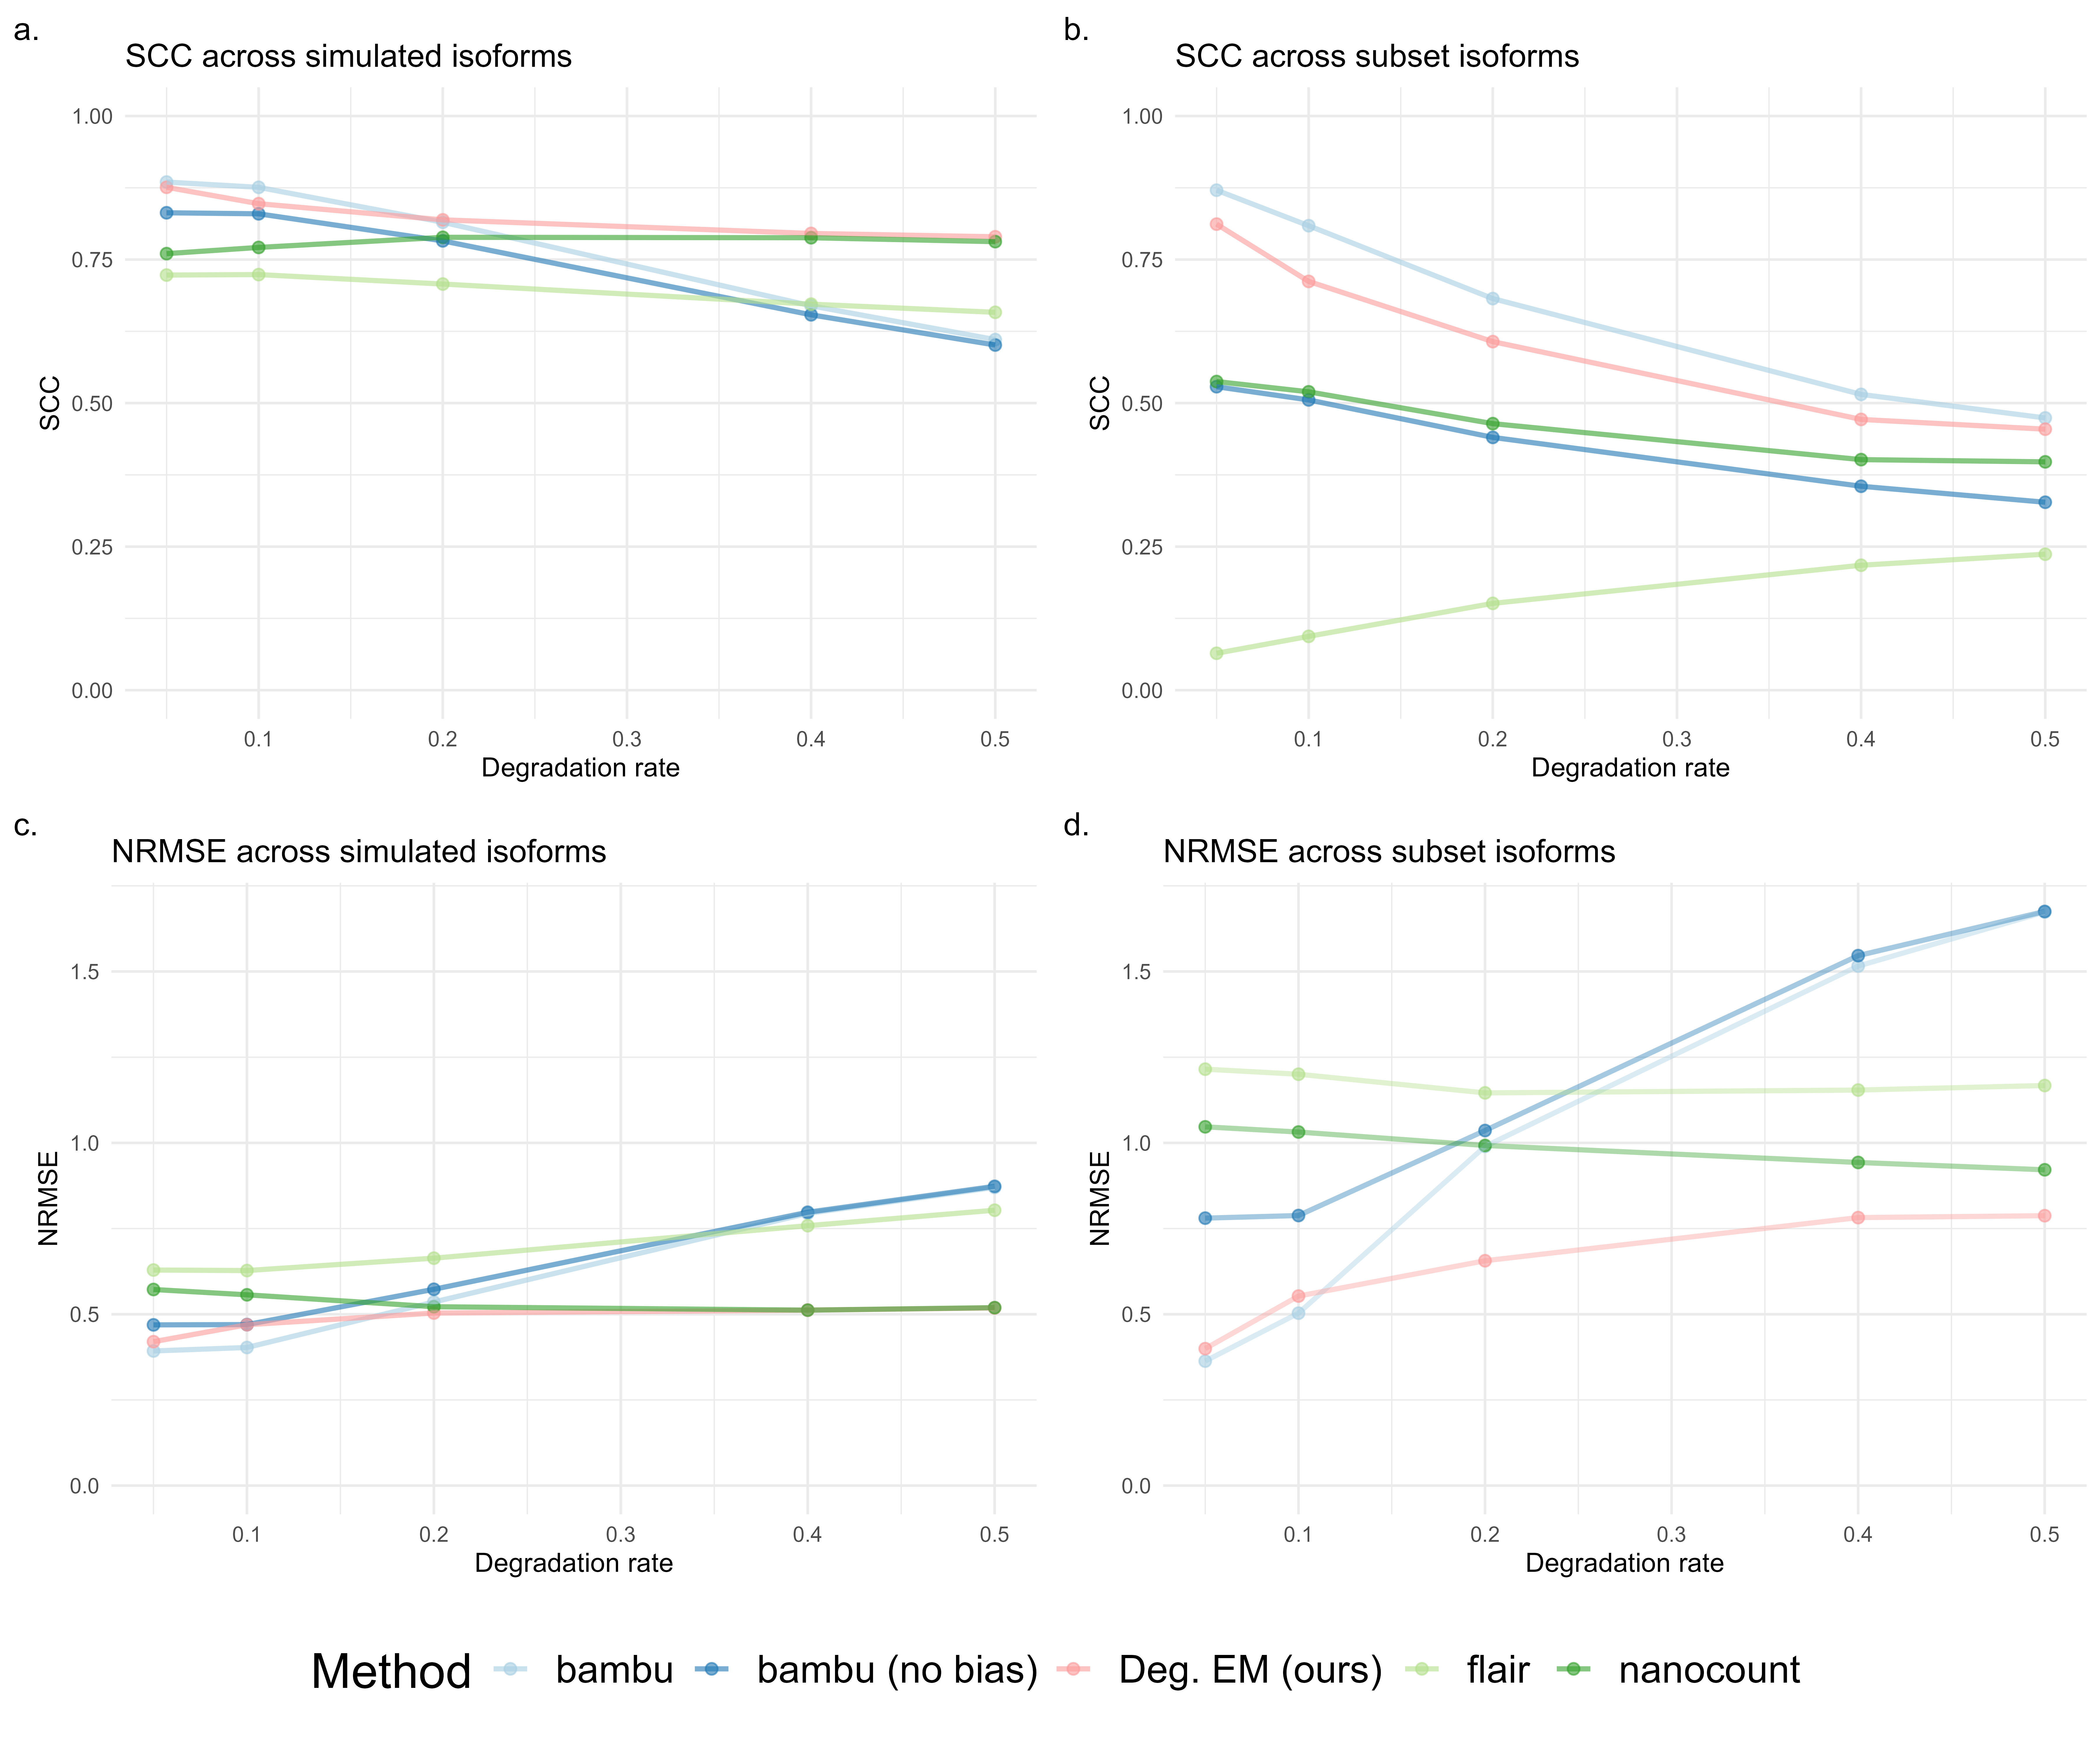
\includegraphics[width=\textwidth]{figures/sec-3-scc-nrmse.png}
    \caption{Caption}
    \label{fig:my_label}
\end{figure}

\begin{figure}[H]
    \centering
    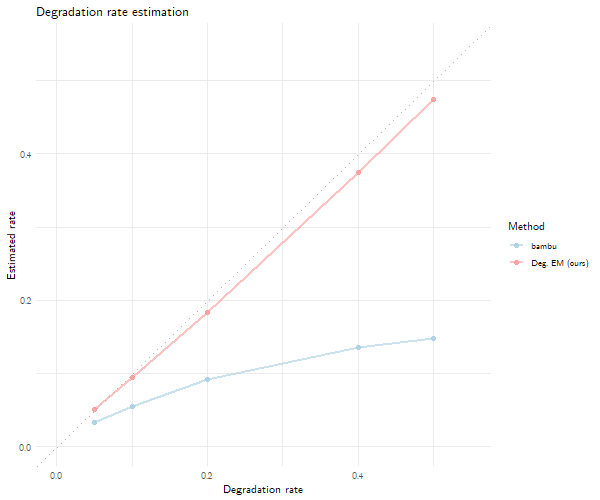
\includegraphics[width=0.7\textwidth]{figures/sec-3-deg-est.png}
    \caption{Caption}
    \label{fig:my_label}
\end{figure}